\chapter{The Actor Model for the Compute Continuum}
\label{chap:actor_model}

Computing infrastructures in 2024 are characterized by strong \textbf{pervasiveness}, we are surrounded by them, and computations happen everywhere anytime.

This is the \textbf{Compute Continuum}, a concept that describes the continuous interaction between the physical and digital worlds, and the seamless integration of the digital world into the physical world.

\section{Towards the Actor Model}

Given the strong decentralization of the Compute Continuum, the need for a decentralized computational models became strong.

The \textbf{Actor Model} is a computational model for decentralized concurrent computation that treats \ul{actors as the universal primitives of concurrent computation}. 
In response to a message that it receives, an actor can make local decisions, create more actors, send more messages, and determine how to respond to the next message received. \ul{Actors may modify their own private state, but can only affect each other indirectly through messaging} (removing the need for locks).

{This model nicely fits modern computing challenges:\ns
\begin{itemize}
   \item Self-organisation programming
   \item Collective adaptive systems
   \item Cyber-physical systems and IoTs
   \item Edge and fog computing
\end{itemize}}

Fun fact, the Actor Model was first proposed by Carl Hewitt in 1973, and it was inspired by the work of Alonzo Church on the \textit{Lambda Calculus}, it was oriented for implemeting AI.

\subsection{MapReduce - Why not?}
The key issue is that MapReduce does not fit well scenarios where we don't know the number of steps in advance, or where we don't know where the computation will take place.
In general MapReduce is not a good fit for heterogeneous environments.

However, we will see that the MapReduce is an instance of a more general concept/model: the \textit{Bulk Synchronous Parallel} model.

\section{BSP - Bulk Synchronous Parallel model}
This model is a \textit{bridging model} for designing parallel algorithms.
{It defines three global super-steps:\ns
\begin{enumerate}
   \item Concurrent computation
   \item Communication
   \item Barrier synchronization
\end{enumerate}}

The problem with having a full synchronization at the end, is that reliability and network partitioning can cause the system to hang a lot.
This is a more critical issue than latency, throughput, and bandwidth.

\section{Delegation}
In order to reach the scalability we are looking for we want model that are by design decentralized.

\begin{itemize}
   \item Actor Based models and frameworks
   \begin{itemize}
      \item Akka - Java/Scala based, no longer OpenSource
      \item Orleans - .NET based
      \item CAF - C++ based
      \item Ray - Python based
      \item ZIO Actors - Scala based, oriented for computations happening in a single machine
   \end{itemize}
   \note{This is the model used by the Halo 4 backend}
   \item Reactive programming - paradigm that emphasizes the use of asynchronous data streams to handle events and data flows.
   \note{Used in the Netflix API}
\end{itemize}

The underlying architecture is typically not simply threads, because a single machine may also manage millions of actors, and threads are not a good fit for this scenario.
Actors may be organized, for instance in a list, and a single thread may invoke them in a round-robin fashion.
We could also have multiple threads, handling such lists of actors; there are many possible implementations.



\section{The Actor Model - Key Concepts}

\begin{figure}[htbp]
   \centering
   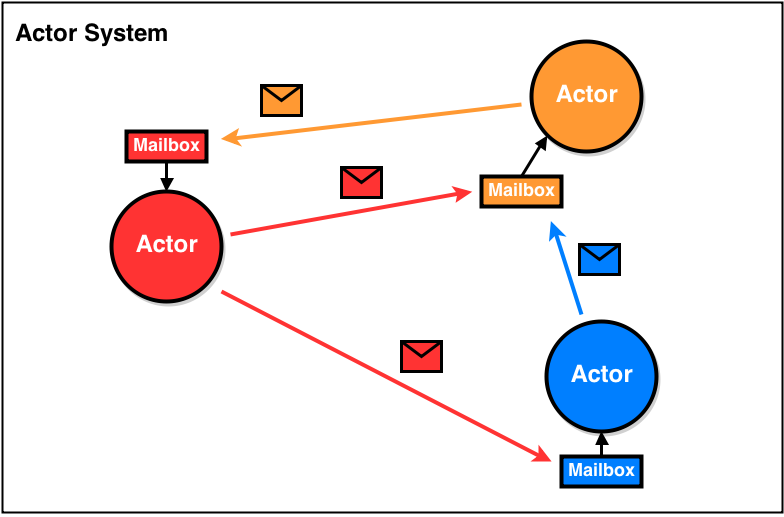
\includegraphics{images/15/actormodel.png}
   \caption{Actor model schema}
   \label{fig:15/actormodel}
\end{figure}

The actor model provides a simple and intuitive programming model for building highly concurrent and distributed systems.

It emphasizes message passing and actor isolation, which helps to improve the modularity and scalability of the system.

\begin{definition}
   [Actor]
   An actor is a computational entity that, in response to a message it receives, can concurrently:\ns
   \begin{itemize}
      \item send a finite a number of messages to other Actors
      \item create a finite number of new Actors
      \note{Enables to model to express any degree of concurrency}
      \item designate the behavior to be used for the next message it receives
      \note{Actors are not \textit{stateless}, and keep track of the progress of the computation}
   \end{itemize}
\end{definition}

Modularity in the Actor model comes from one-way asynchronous communication. Once a message has been sent, it is the responsibility of the receiver.

Messages in the Actor model are decoupled from the sender and are delivered by the system on a best-effort basis.


Note also that since Actors can create new Actors, they implicitly create a hierarchical relation between them, allowing to exploit the locality of the computation.

\subsection{Indeterminacy and quasi-commutativity}
Messages are delivered asynchronously, and the order of delivery is not guaranteed, hence, \ul{the actor model is \textbf{not} completely \textbf{deterministic}}.

\textbf{Quasi-commutativity} is a property of the actor model that states that the \textit{order} of messages sent by an actor to another actor does \textit{not} affect the outcome of the computation (in some cases).\\
In other words, there must be some flexibility concerning the order of messages, to avoid making the system obey a strict order of messages dictated by delays, errors, and lost messages.

\subsection{Fault tolerance and Scalability}
The actor model is inherently fault-tolerant, as the failure of one actor does not prevent the rest of the system from functioning, besides, actor may be restarted or moved to another machine in case of failure.\\
Furthermore, it provides a scalable approach to building systems by allowing actors to be dynamically created and distributed across multiple machines, enabling systems to scale horizontally by adding more machines to handle increasing loads.\
This is even simplified by the absence of primitives such as locks and semaphores, reducing the risk deadlocks, race conditions and bootlenecks due to busy waiting.
One-way asynchronous communication allows all this.

\textbf{Self-organising} systems, as well as \textbf{adaptive} systems, may be built using the actor model framework, where actors can adapt their behavior based on the state of the system and the messages they receive, aiming at a global goal.\
Not to mention IoTs where, essentially, each device may be implemented as an actor.

\subsection{Challenges}

\begin{itemize}
	\item \textbf{Complexity}: Designing and implementing actor-based systems can be complex
	\item \textbf{Testing}: Testing and debugging actor-based systems can be challenging due to their concurrent and asynchronous nature. It can be difficult to reproduce and isolate bugs that arise from race conditions
	\item \textbf{Overhead}: The actor model adds some performance overhead due to the need to manage and schedule actors, and the cost of message passing between actors
	\item \textbf{Consistency}: Ensuring consistency and coordination between actors can be challenging, especially when dealing with distributed systems where actors may be running on different machines or in different data centres.
	\item \textbf{Integration}: Integrating actor-based systems with existing systems and technologies can be challenging, especially when dealing with legacy systems or systems that use different programming languages or platforms.
\end{itemize}